\documentclass{article}
\usepackage[T1]{fontenc}
\usepackage{lmodern}
\usepackage{graphicx}
\usepackage{amsmath,amssymb}
\usepackage[a4paper,margin=2cm]{geometry}
\usepackage[absolute,overlay]{textpos}
\setlength{\TPHorizModule}{1mm}
\setlength{\TPVertModule}{1mm}
\usepackage[indonesian]{babel}
\usepackage{hyperref}
\setlength{\emergencystretch}{2em}
% unit: Halaman 58

\begin{document}

% === Halaman 58 (llm) ===

\begin{itemize}
    \item Di dalam beberapa \textit{cipher} blok, permutasi direalisasikan dengan menggunakan matriks permutasi yang dinamakan $P$-box. Entri di dalam $P$-box menyatakan bit dari posisi sebelumnya.
    \item Contoh P-box di dalam DES:
\end{itemize}

\vspace{10mm}

Artinya, bit ke 58 dari bit-bit input dipindahkan ke posisi pertama, bit ke-50 pada posisi kedua, dst

\vspace{10mm}

\begin{itemize}
    \item Beberapa skema permutasi juga melakukan kompresi (mengurangi bit-bit input) atau ekspansi (memperbanyak bit-bit) pada operasi permutasi.
\end{itemize}

% deskripsi: Tabel matriks P-box DES yang berisi angka-angka posisi bit.
% bbox normalisasi: [0.1000, 0.3100, 0.9600, 0.5100]
\begin{textblock*}{180.60mm}(21.00mm,92.07mm)
\noindent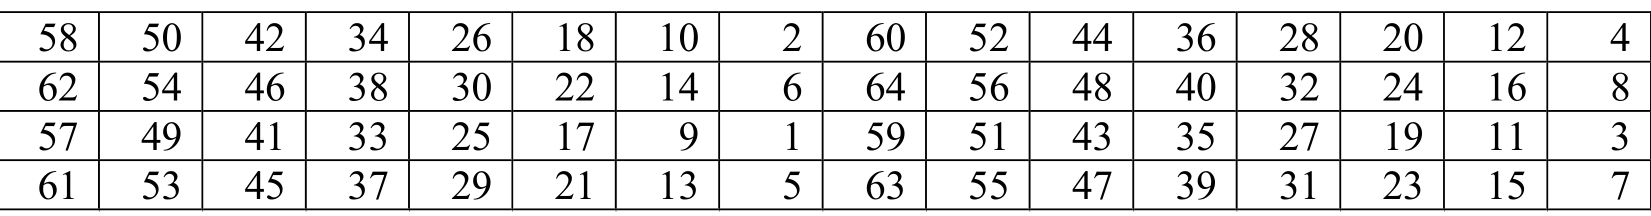
\includegraphics[width=180.60mm,height=59.40mm]{../../images/llm/page_058_img_01.png}%
\end{textblock*}

% deskripsi: Diagram ilustrasi proses ekspansi bit dari input 'Right Half i-1' menjadi deretan bit yang lebih panjang.
% bbox normalisasi: [0.8000, 0.7800, 0.9600, 0.9200]
\begin{textblock*}{33.60mm}(168.00mm,231.66mm)
\noindent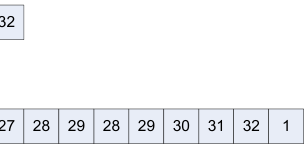
\includegraphics[width=33.60mm,height=41.58mm]{../../images/llm/page_058_img_02.png}%
\end{textblock*}

\end{document}
